\section{提案手法1}
\subsection{\rm EEG \mc データ}
実験データとしてBCI2000システム\cite{BCI2000}を用いて記録された
PhysioNet\cite{PhysioNet}が提供する運動想起データセットを用いた。
電極の配置は標準的な10-10システム(図\ref{fig:10system})であり、サンプリング周波数は160Hzである。
109人の被験者が定められたタイムスケジュールに従い、
左手、右手、両手および両足の運動想起を行っている。
運動想起のタイムスケジュールを表す図を図\ref{fig:motorimage}に示す。
運動想起の開始時には被験者の前面に配置されたディスプレイから
右手あるいは左手の運動想起の指示が出される。
被験者は4秒間指示された手の
指を開いたり閉じたりする運動想起試行を続け、その後4.2秒間の休息時間が与えられる。
休息時間を終えると再びディスプレイから両手あるいは両足の運動想起の指示が出され、
被験者は4秒間の支持された部位の指を開いたり閉じたりする運動想起試行を行う。その後4.2秒の休息時間が再び与えられる。
計16.4秒を1サイクルとし、被験者1人につき45サイクルを繰り返し行う。
従って被験者は左手、右手、両手、両足で計90回の運動想起を行っている。

PhysioNetが提供する運動想起時のEEGデータベースは、
世界最大規模の被験者数を有している。
また、EEGの計測時に用いられたBCI2000システムは運動想起型BCIのみならず、
多種多様なBCIシステムを構築するために公開されたプログラム群であり、
多くの脳研究者に利用されている。
従って、手法の評価と検討を行うためのデータとして信頼性が高いと考えたため利用した。

\begin{figure}[t]
    \centering
    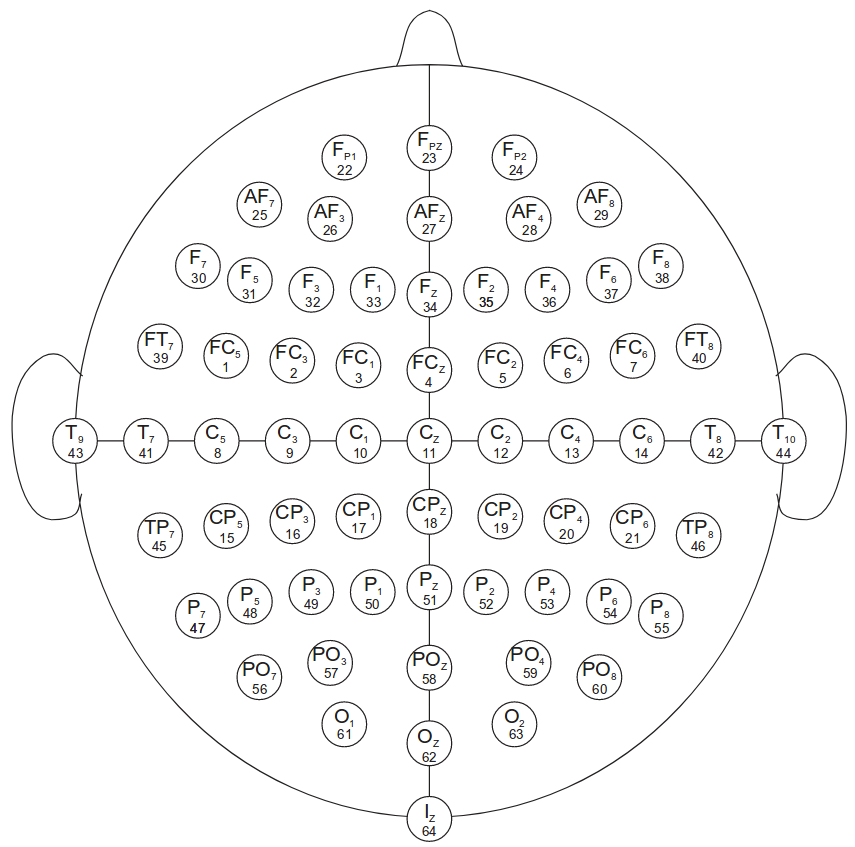
\includegraphics[width=12cm]{images/system1010.png}
    \caption{10-10システムの電極配置}
    \label{fig:10system}
\end{figure}
\begin{figure}[t]
    \centering
    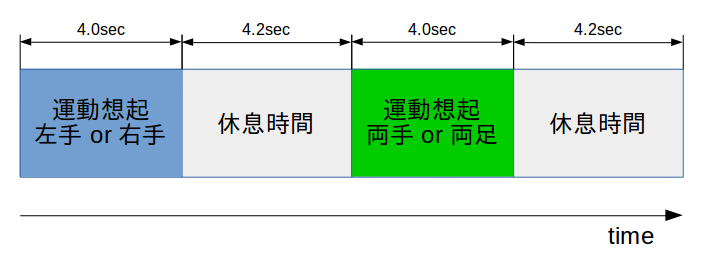
\includegraphics[width=12cm]{images/motorimage.png}
    \caption{運動想起EEG測定のタイムスケジュール}
    \label{fig:motorimage}
\end{figure}


\subsection{評価方法}
本研究では各運動想起時間である4秒間のデータを取り出して、
2クラス分類の問題を\(_4C_2=6\)種類準備した。
ここで運動想起は一人あたり計90回行っており4部位あるため、
1つの部位につき22回あるいは23回の試行が行われている。
従って準備した2クラス問題におけるデータ数は44〜46となっている。
また、以降2クラス分類の問題は表\ref{table:pattern}に示す通り表記する。
\begin{table}[t]
    \centering
    \caption{分類問題の種類と論文内の表記}
    \begin{tabular}{|c|c|} \hline
        分類問題 & 論文内の表記 \\ \hline
        左手or右手 & LR \\ \hline
        両手or両足 & HF \\ \hline
        左手or両手 & LH \\ \hline
        左手or両足 & LF \\ \hline
        右手or両手 & RH \\ \hline
        右手or両足 & RF \\ \hline
    \end{tabular}
    \label{table:pattern}
\end{table}
問題LRを例にする。
ニューラルネットワークは4秒間のEEGデータを受け取り、
LかRかのいずれかを出力するように構成する。
EEGデータの与え方及びニューラルネットワークの構成を
被験者や問題ごとに変更を行わないことで、
単一のニューラルネットワークが被験者に関わらず、また
問題に関わらずBCIを構成可能かを評価する。

また評価指標としては正解率を用いる。
正解率はニューラルネットワークがEEGを元に出力する分類結果と、
EEG計測時に被験者が行った運動想起が一致している割合である。
また、評価に用いられるEEGは学習には用いていないデータである。
被験者は99人とし、それぞれ6つの分類問題が準備されているため計594の
正解率が得られる。594の正解率はそれぞれ10-交差検証によって算出する。
各問題について99人の被験者の正解率の平均を取ることで、
単一のニューラルネットワークが各問題に適応可能かを評価する。

\subsection{ニューラルネットワークの構成}
n階のテンソル\(A\in \mathbb R^{D_1,\cdots ,D_n}\)の
\((d_1,\cdots,d_n)\)成分を\(a_{d_1,\cdots,d_n}\)と表記する。
入力\(X \in \mathbb R^{M\times N\times C}\)に対して
Convolution層のパラメータを\(H \in \mathbb R^{P\times Q \times C \times L}\)として
\begin{equation}
    u_{m,n,k} = \sum_{c=1}^C\sum_{p=0}^{P-1}\sum_{q=0}^{Q-1} x_{m+p,n+q,c} h_{p,q,c,k} + b_{m,n,k}
\end{equation} 
と計算する。
ここでテンソルの各次元について\(X \in \mathbb R^{space\times time\times frequency}\)であると仮定する。
提案手法のニューラルネットワークの構成は入力側から
\begin{enumerate}
    \item 畳み込み層\(H_1 \in \mathbb R^{75\times 1 \times 1 \times 32}\)
    \item 畳み込み層\(H_2 \in \mathbb R^{1\times 64 \times 32 \times 64}\)
    \item バッチ正規化
    \item 平均プーリング1(プーリングサイズ:75とストライド:25)
    \item ドロップアウト
    \item \(H_3 \in \mathbb R^{12\times 1 \times 64 \times 2}\)
    \item 平均プーリング2(出力サイズが\(1\times 1\times 2\)となるように設定)
    \item ソフトマックス
\end{enumerate}
とした。
損失関数としては交差エントロピー関数を用いた。
最適化法としては比較的収束が速いとされるAdamを利用した。
ドロップアウト率は0.5であり、\(L_1\)正則化や\(L_2\)正則化などの手法は用いていない。
平均プーリング1はtime方向のみに行った。
平均プーリング2は出力の要素数が\(2\)になるように調整し、
各要素が2クラス分類におけるlogitを出力するようにした。


\subsection{結果}
各分類問題における正解率のヒストグラムを示す(図\ref{fig:LRhist}-\ref{fig:RFhist})。
横軸が正解率で、縦軸が被験者の数である。
どの分類問題においても60〜70\%付近の正解率となる被験者が多い。
一方で、80\%以上の正解率となる被験者から50\%の正解率となる被験者までいる。

\begin{figure}[t]
    \begin{minipage}{0.5\hsize}
     \begin{center}
      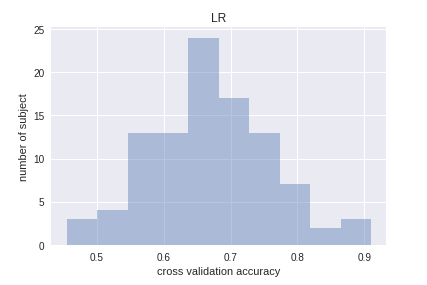
\includegraphics[width=80mm]{images/LR.png}
     \end{center}
     \caption{LR問題の正解率ヒストグラム}
     \label{fig:LRhist}
    \end{minipage}
    \begin{minipage}{0.5\hsize}
     \begin{center}
      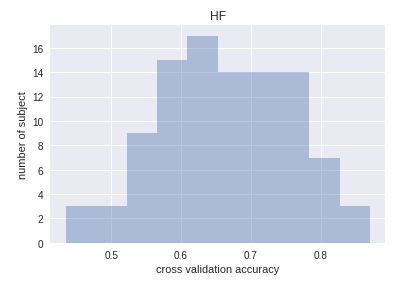
\includegraphics[width=80mm]{images/HF.png}
     \end{center}
     \caption{LR問題の正解率ヒストグラム}
     \label{fig:HFhist}
    \end{minipage}
\end{figure}
\begin{figure}[t]
    \begin{minipage}{0.5\hsize}
     \begin{center}
      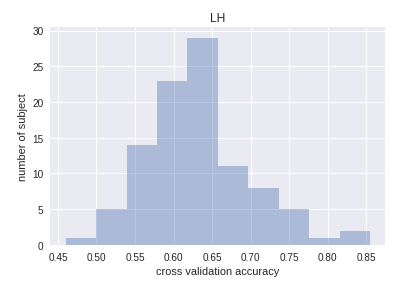
\includegraphics[width=80mm]{images/LH.png}
     \end{center}
     \caption{LH問題の正解率ヒストグラム}
     \label{fig:LHhist}
    \end{minipage}
    \begin{minipage}{0.5\hsize}
     \begin{center}
      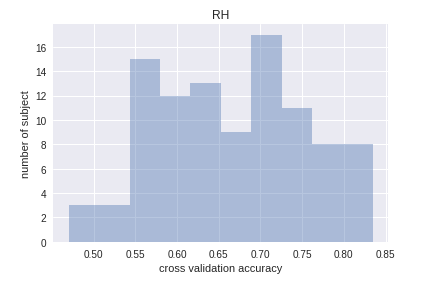
\includegraphics[width=80mm]{images/RH.png}
     \end{center}
     \caption{RH問題の正解率ヒストグラム}
     \label{fig:RHhist}
    \end{minipage}
\end{figure}
\begin{figure}[t]
    \begin{minipage}{0.5\hsize}
     \begin{center}
      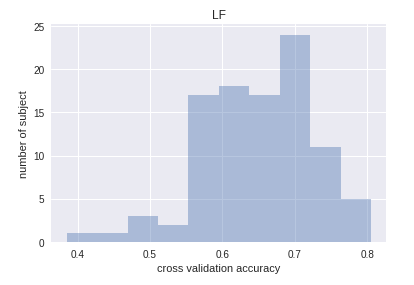
\includegraphics[width=80mm]{images/LF.png}
     \end{center}
     \caption{LF問題の正解率ヒストグラム}
     \label{fig:LFhist}
    \end{minipage}
    \begin{minipage}{0.5\hsize}
     \begin{center}
      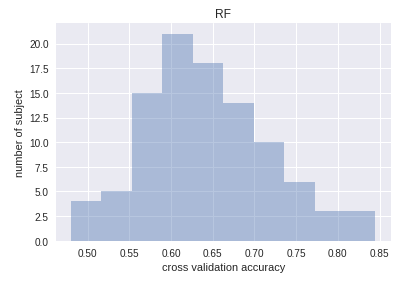
\includegraphics[width=80mm]{images/RF.png}
     \end{center}
     \caption{RF問題の正解率ヒストグラム}
     \label{fig:RFhist}
    \end{minipage}
\end{figure}

各分類問題における全被験者の平均を表\ref{table:meanacc}に示す。
分類問題毎の平均の差異は小さく、タスクに依らず一定の性能を確保できることが分かる。
しかし、この結果はバタワースバンドパスフィルタと
CSPとLDAを組み合わせた手法\cite{benth}(表\ref{table:meanacc_csp})に対して
性能が高いとは言い難い。
\begin{table}[t]
    \begin{minipage}{0.5\hsize}
        \centering
        \caption{提案手法の問題毎の平均}
        \begin{tabular}{|c|c|} \hline
            分類問題 & 平均正解率 \\ \hline
            LR & 0.6712 \\ \hline
            HF & 0.6636 \\ \hline
            LH & 0.6322 \\ \hline
            LF & 0.6643 \\ \hline
            RH & 0.6517 \\ \hline
            RF & 0.6427 \\ \hline
        \end{tabular}
        \label{table:meanacc}
    \end{minipage}
    \begin{minipage}{0.5\hsize}
        \centering
        \caption{従来手法の問題毎の平均}
        \begin{tabular}{|c|c|} \hline
            分類問題 & 平均正解率 \\ \hline
            LR & 0.6124 \\ \hline
            HF & 0.7719 \\ \hline
            LH & 0.7760 \\ \hline
            LF & 0.8093 \\ \hline
            RH & 0.8196 \\ \hline
            RF & 0.6701 \\ \hline
        \end{tabular}
        \label{table:meanacc_csp}
    \end{minipage}
\end{table}

\subsection{考察}
表\ref{table:meanacc} によると提案手法1のニューラルネットワークは
いずれの問題に対しても平均的には同等の対応力を有するように捉えられる。
しかし図\ref{fig:LRhist}-\ref{fig:RFhist}からは、
問題ごとに異なったヒストグラムが得られており任意のタスクに対して
同等に学習が可能であるとは言い難い。
また、問題LR以外は従来手法よりも性能が劣っている。

このような結果となった理由として、
実験に対して一回の学習に用いるデータ数が高々40個程であったことが
問題であると考える。
従来手法の最適化は第2章で述べた通り、解析的に実行が可能である。
また凸最適化問題であるため、BCIの構成要素1つ1つは
仮定した関数族の中で最適であることが保証されている。
従って、与えられた分類問題に有効な入出力関係を包含する関数族となっていれば、
極めて高い性能を保証することができる。
一方でニューラルネットワークの学習は一般的に非凸の最適化問題であり、
逐次的な最適化方法を用いなければならない。
学習データが少ない場合は逐次最適化で得られる勾配のバリエーションが乏しくなり、
探索範囲が極めて狭くなってしまうと推察できる。

一般にニューラルネットワークが表現できる関数の集合は非常に大きい。
すなわち提案した手法は分類問題に有効な入出力関係を包含する関数族となっているはずである。
しかし、学習データが少ない場合には大きな関数の集合の中を十分に探索することができない。
この考察を確認するために以下の追加実験を行った。

\subsection{追加実験とその結果}
追加実験ではLR問題のみを扱った。
LR問題のデータを50人分集めすべてのデータを統合し、2200個へと増加させた。
すなわち左手の運動想起が1100回分と右手の運動想起が1100回分準備されたことになる。
このデータに対して10-交差検証によって正解率を算出した。
この時にもニューラルネットワークの構造やハイパーパラメータの調整は行っていない。

結果として交差検証の平均正解率は0.8032となった。
この結果は個々の人間に対して学習させた正解率の結果よりも向上している。
すなわち、学習データの増加がニューラルネットワークの性能を引き上げたことが分かる。
また、50人すべてのLR問題に対応できるようにニューラルネットワークが学習を行っている点で、
個人事に学習したニューラルネットワークよりも難しいタスクをこなしていると言える。

また表\ref{table:allvalidation}に10回の検証のそれぞれの正解率を示した。
各検証では50人の被験者のデータからランダムに220個のデータが検証データに用いられ、
残りの1980個のデータが学習データとして用いられている。
どのような組み合わせで学習が行われても75\%以上の高い性能を発揮しており、
人類に共通したBCIモデルの構築の可能性を示唆している。
\begin{table}[t]
    \centering
    \caption{10交差検証の内訳}
    \begin{tabular}{|c|c|c|c|c|c|c|c|c|c|} \hline
        検証1 & 検証2 & 検証3 & 検証4 & 検証5 &
        検証6 & 検証7 & 検証8 & 検証9 & 検証10 \\ \hline
        0.8318 & 0.8136 & 0.7909 & 0.7955 & 0.7909 &
        0.7500 & 0.8090 & 0.8318 & 0.8045 & 0.8136 \\ \hline
    \end{tabular}
    \label{table:allvalidation}
\end{table}
